\documentclass[12pt]{article}
\usepackage[utf8]{inputenc}

\title{Analysis and Design of Algorithms}
\author{}
\date{April 2019}

\usepackage{natbib}
\usepackage{graphicx}
\usepackage{hyperref}
\usepackage{listings}

\begin{document}

\maketitle

\section{Warm up}

Lets modify the classic merge sort algorithm a little bit. What happens if instead of splitting the array in 2 parts we divide it in 3? You can assume that exists a three-way merge subroutine. What is the overall asymptotic running time of this algorithm?

\emph{BONUS:} Implement the three-way merge sort algorithm.\\

\textbf{Solution:}\\
The execution time of the traditional merge sort is of\begin{equation} cn (log2 (n) +1) \end{equation} , but when divided into 3 subprocesses, this would change to a time of execution of \begin{equation} cn (log3 (n) +1) \end{equation} being more optimal than the traditional.\\\\
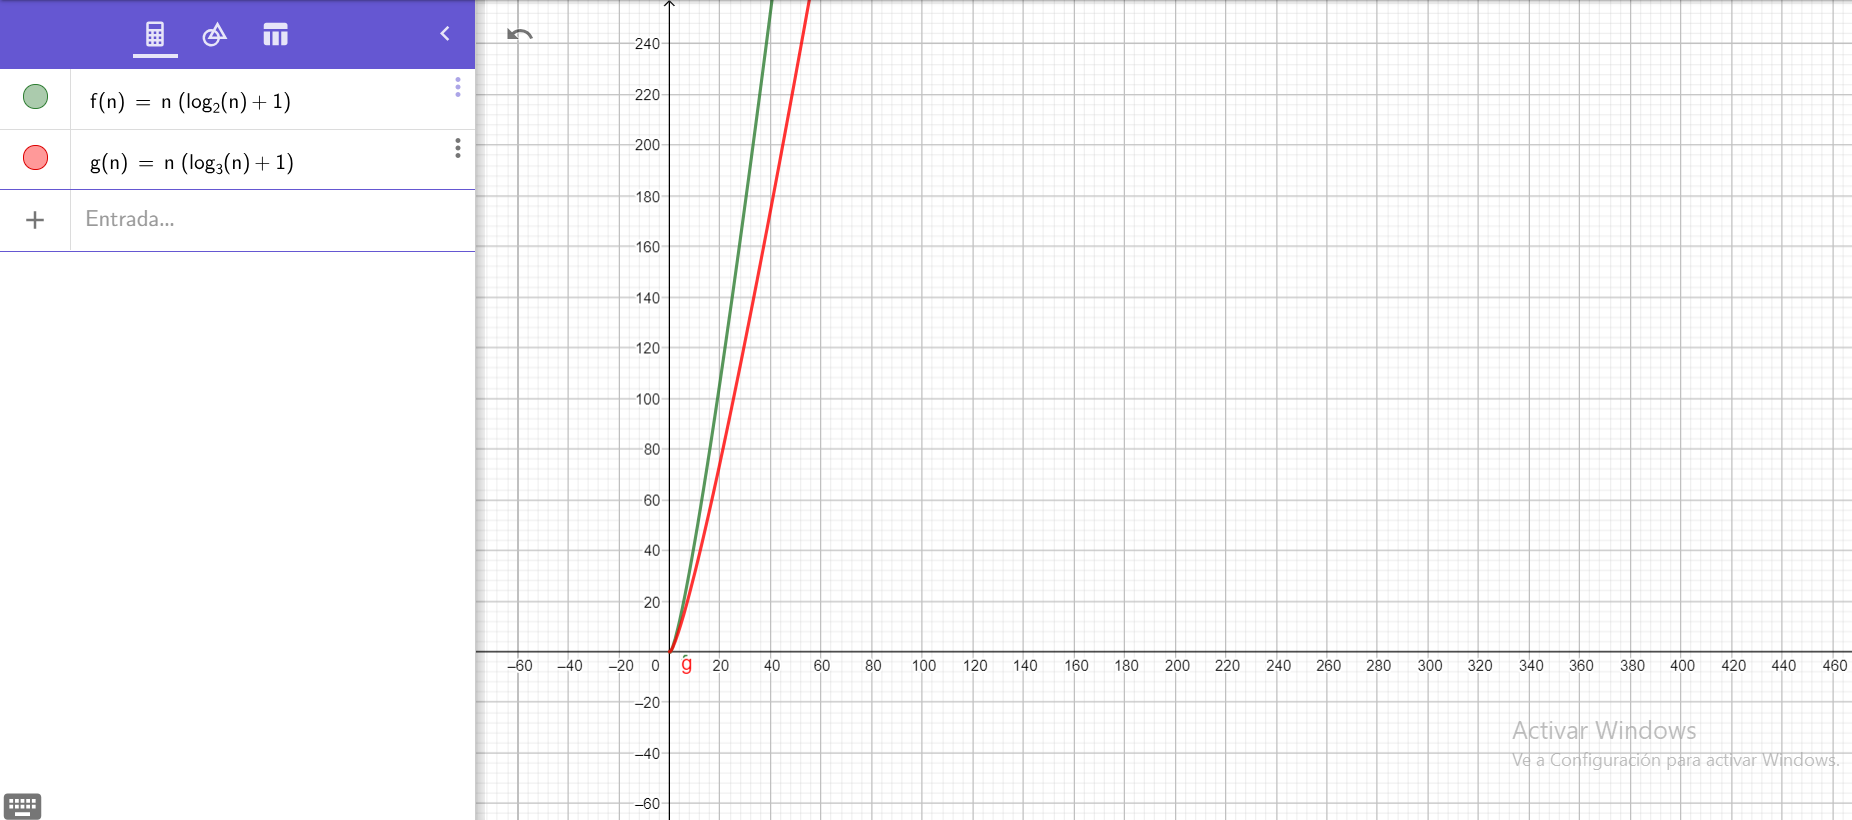
\includegraphics[width=8cm, height=6cm]{Captura}
\centering
\section{Competitive programming}

Welcome to your first competitive programming problem!!! 

\begin{itemize}
    \item Sign-up in Uva Online Judge (\url{https://uva.onlinejudge.org}) and in CodeChef if you want (we will use it later).
    \item Rest easy! This is not a contest, it is just an introductory problem. Your first problem is located in the ``Problems Section'' and is \textbf{100 - The 3n + 1 problem}.
    
    \item Once that you finish with that problem continue with \textbf{458 - The Decoder}. Again, this problem is just to build your confidence in competitive programming.
    
    \item \emph{BONUS:} \textbf{10855 - Rotated squares}\\
    
\textbf{Solution:}\\
\textbf{The 3n + 1 problem:}\\
\lstinputlisting[language=c++]{100.cpp}
////////////////////////////////////////////////////////////////////////////// \\
\textbf{The Decoder:}\\
\lstinputlisting[language=c++]{458.cpp}
    
\end{itemize}

\section{Simulation}

Write a program to find the minimum input size for which the merge sort algorithm always beats the insertion sort.

\begin{itemize}
    \item Implement the insertion sort algorithm
    \item Implement the merge sort algorithm
    \item Just compare them? No !!! Run some simulations or tests and find the average input size for which the merge sort is an asymptotically ``better'' sorting algorithm.
\end{itemize}

Note: Include (.tex) and attach(.cpp) your source code and use a dockerfile to interact with python and plot your results.\\

\emph{BONUS:} Compare both algorithms against any other sorting algorithm

\section{Research}

Everybody at this point remembers the quadratic ``grade school'' algorithm to multiply 2 numbers of $k_{1}$ and $k_{2}$ digits respectively. \\

Your assignment now is to compare the number of operations performed by the quadratic grade school algorithm and Karatsuba multiplication.

\begin{itemize}
    \item Define Karatsuba multiplication
    \item Implement grade school multiplication
    \item Implement Karatsuba multiplication
    \item Compare Karatsuba algorithm against grade school multiplication
    \item Use any of your implemented algorithms to multiply $a*b$ where:
    \begin{description}
    \item{a:} 3141592653589793238462643383279502884197169399375105820974944592
    \item{b:} 2718281828459045235360287471352662497757247093699959574966967627
    \end{description}
\end{itemize}

Note: Include(.tex) and attach(.cpp) your source code, of course.\\

\textbf{Solution:}\\
\lstinputlisting[language=c++]{multiplication.cpp}
////////////////////////////////////////////////////////////////////////////// \\
The Karatsuba algorithm could not be implemented correctly, but the grade-school multiplication works correctly. Theoretically, the Karatsuba algorithm is more optimal than the grade-school multiplication because Kartsuba's running time is \begin{equation} n^{log2 (3)} \end{equation} while the grade-school multiplication is \begin{equation} n^{2} \end{equation}\\
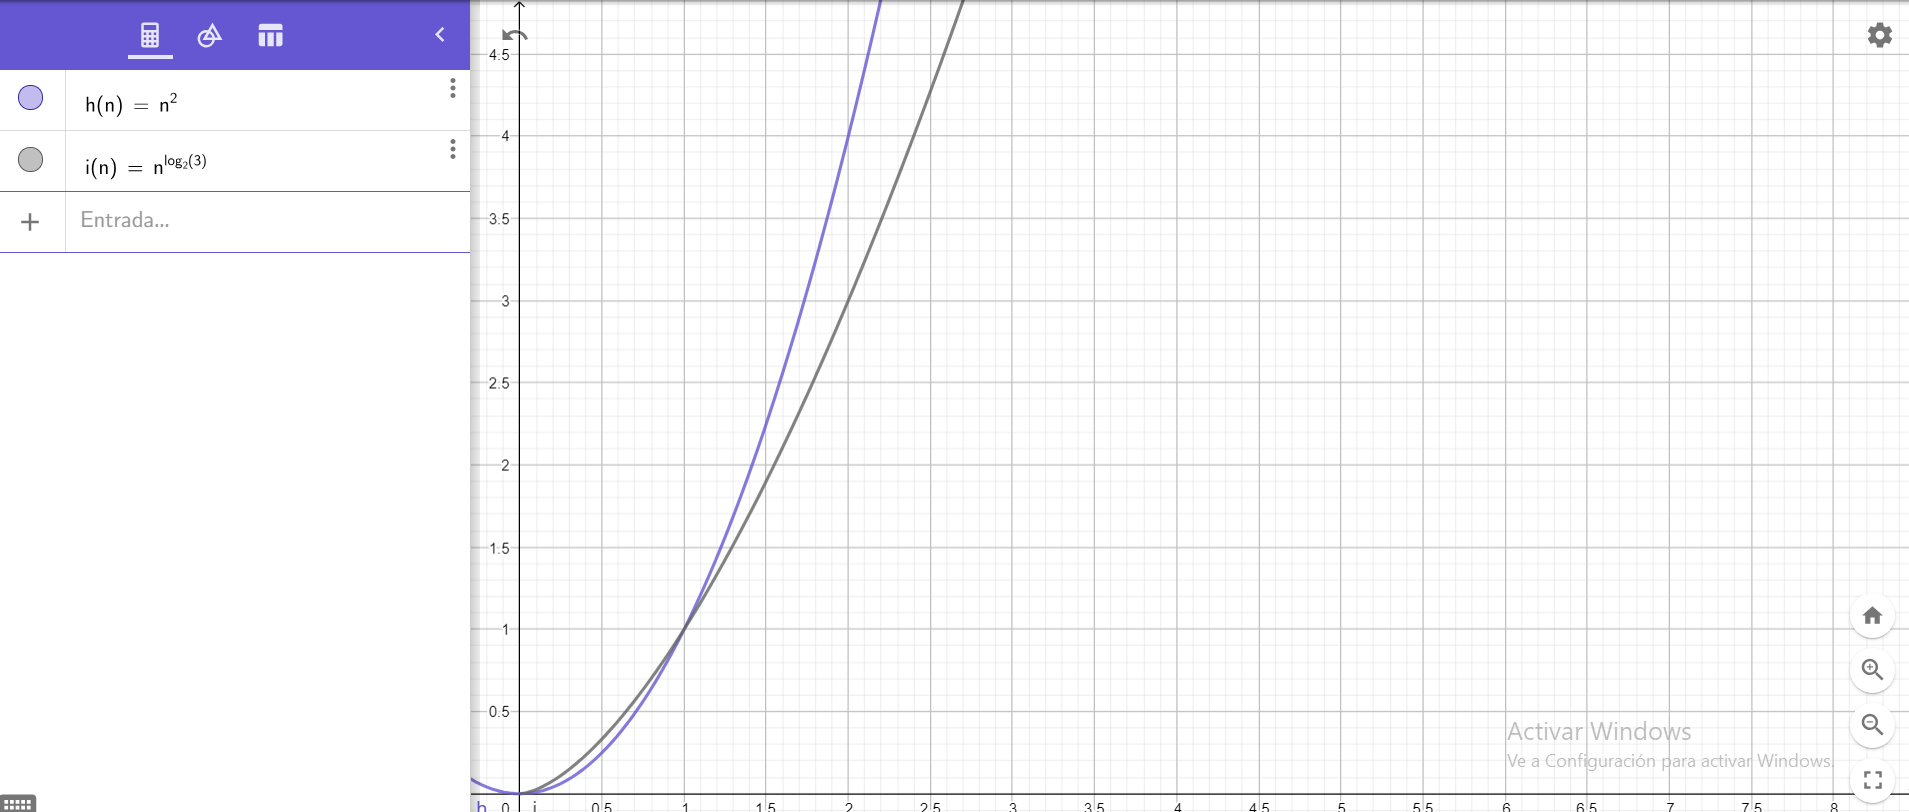
\includegraphics[width=8cm, height=6cm]{2}

\emph{BONUS:} How about Sch\"{o}nhage-Strassen algorithm ? 
\textbf{Solution Bonus:}\\

Theoretically the Schönhage-Strassen algorithm having an execution time of n * log2 (n) * log2 (log2 (n)) is more optimal than the karatsuba algorithm\\\\
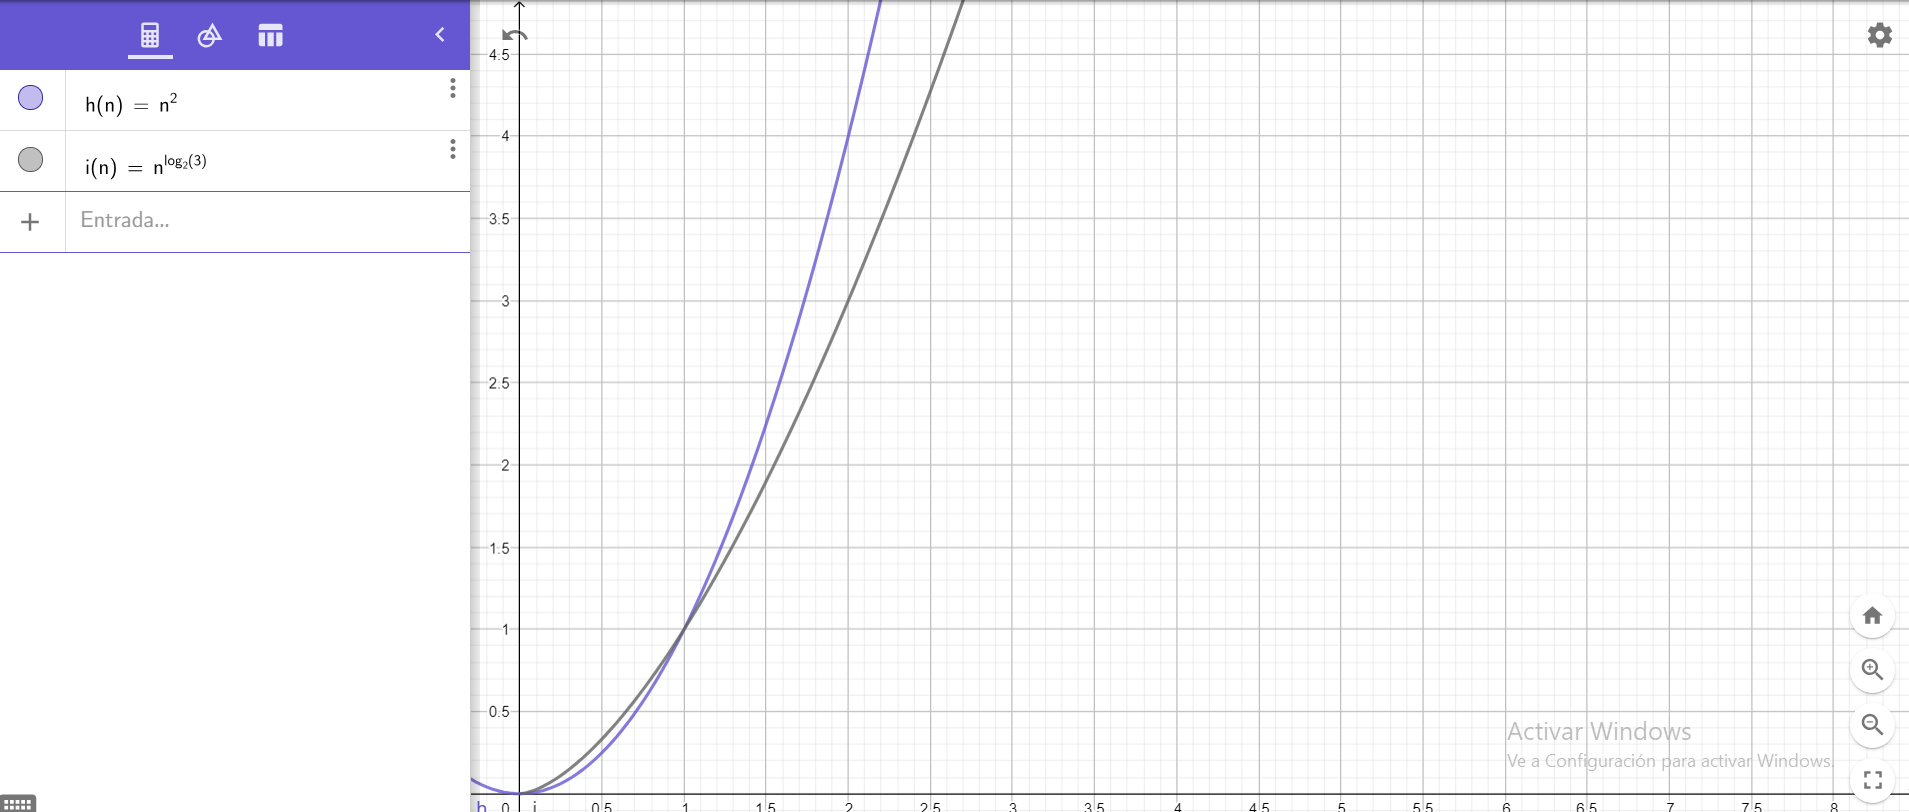
\includegraphics[width=8cm, height=6cm]{2}
\section{Wrapping up}

Arrange the following functions in increasing order of growth rate with $g(n)$ following $f(n)$ if $f(n) = \mathcal{O}(g(n))

\begin{enumerate}
    \item $n^{2}log(n)$
    \item $2^{n}$
    \item $2^{2^{n}}$
    \item $n^{log(n)}$
    \item $n^{2}$
\end{enumerate}
\textbf{Solution:}\\
Ordered from the slowest to the fastest\\
\begin{enumerate}
    \item $n^{2}$
    \item $n^{2}log(n)$
    \item $n^{log(n)}$
    \item $2^{n}$
    \item $2^{2^{n}}$
\end{enumerate}
\end{document}